\section*{Anhang}
\phantomsection
\addcontentsline{toc}{section}{Anhang}

\addtocontents{toc}{\protect\setcounter{tocdepth}{-1}}
\bookmarksetup{depth=-1}

\section{Statische Submodelle des AAS-Demonstrators}
    % In den folgenden Abbildungen sind die im Hauptteil beschriebenen statischen Submodelle der AAS des Abfüll- und Verschließmoduls anhand von Screenshots dokumentiert.
% Sie dienen der Ergänzung und Veranschaulichung der textlichen Beschreibung.
\subsection{Typenschild}
\begin{figure}[H]
    \centering
    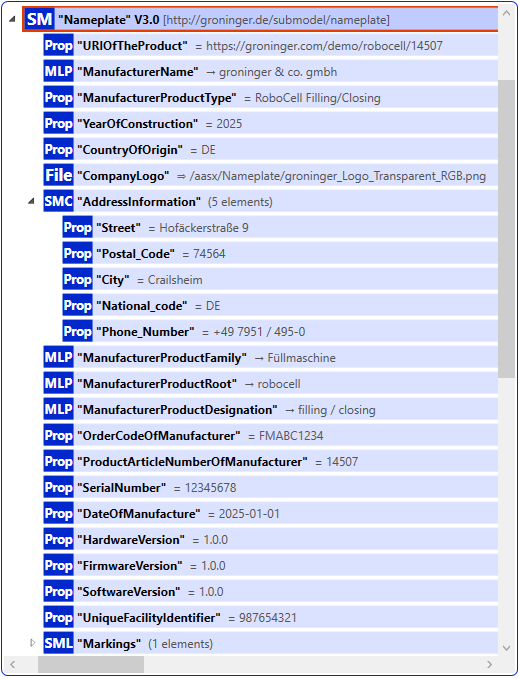
\includegraphics[width=0.9\textwidth]{Bilder/ErgebnissePackageExplorer/Typenschild.PNG}
    \caption{Package Explorer: Submodell Typenschild}
\end{figure}

\newpage
\subsection{Technische Daten}
\begin{figure}[H]
    \centering
    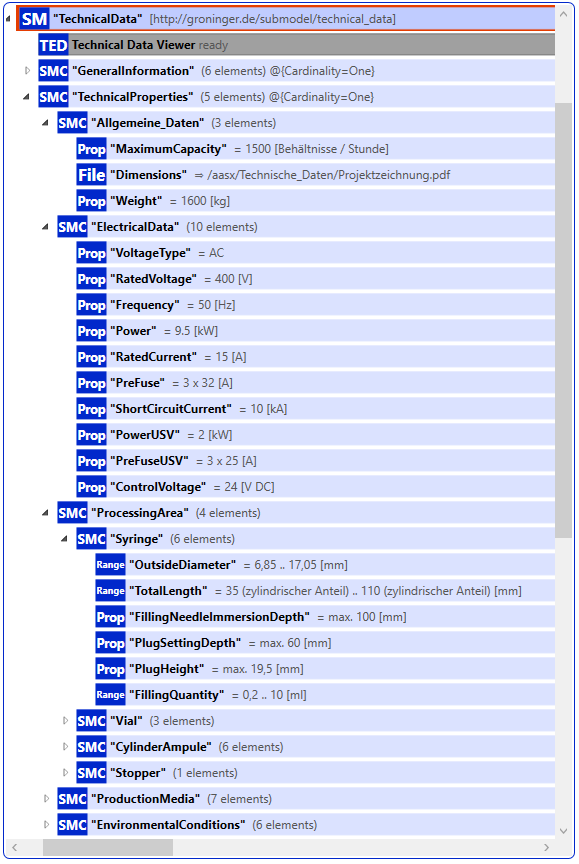
\includegraphics[width=0.9\textwidth]{Bilder/ErgebnissePackageExplorer/TehcnischeDaten.PNG}
    \caption{Package Explorer: Submodell Technische Daten}
\end{figure}

\newpage
\subsection{Dokumentation und 3D-Modelle}
\begin{figure}[H]
    \centering
    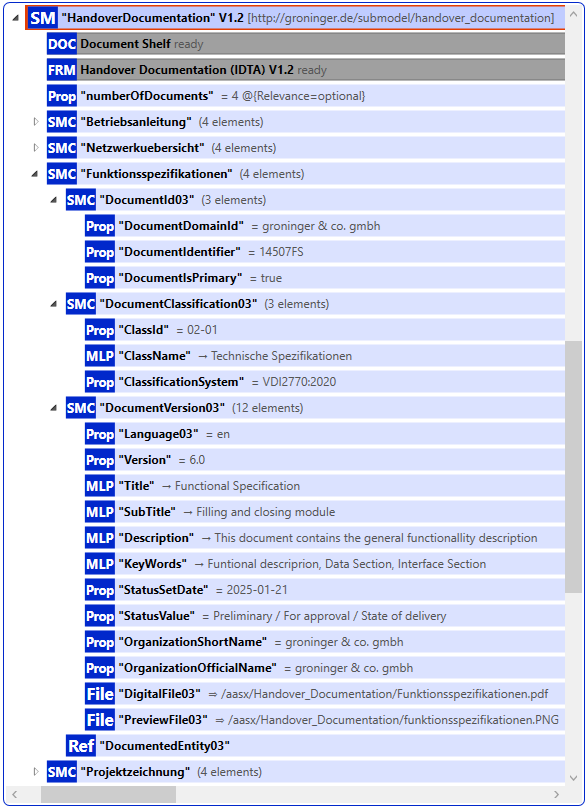
\includegraphics[width=0.9\textwidth]{Bilder/ErgebnissePackageExplorer/SMCDokumentation.PNG}
    \caption{Package Explorer: Submodell Dokumentation (stellvertretend auch für 3D-Modelle)}
\end{figure}

\newpage
\subsection{Wartung}
\begin{figure}[H]
    \centering
    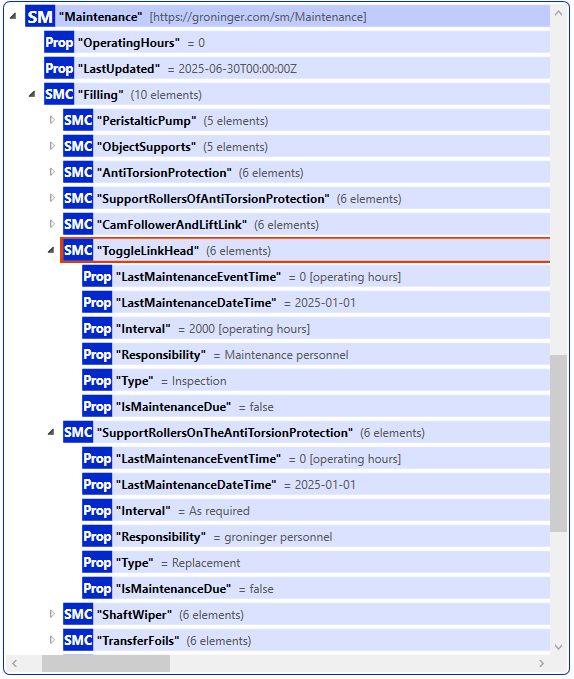
\includegraphics[width=0.9\textwidth]{Bilder/ErgebnissePackageExplorer/Wartung.PNG}
    \caption{Package Explorer: Submodell Wartung}
\end{figure}

\addtocontents{toc}{\protect\setcounter{tocdepth}{2}}
\bookmarksetup{depth=2}